% Options for packages loaded elsewhere
\PassOptionsToPackage{unicode}{hyperref}
\PassOptionsToPackage{hyphens}{url}
%
\documentclass[
]{article}
\usepackage{amsmath,amssymb}
\usepackage{iftex}
\ifPDFTeX
  \usepackage[T1]{fontenc}
  \usepackage[utf8]{inputenc}
  \usepackage{textcomp} % provide euro and other symbols
\else % if luatex or xetex
  \usepackage{unicode-math} % this also loads fontspec
  \defaultfontfeatures{Scale=MatchLowercase}
  \defaultfontfeatures[\rmfamily]{Ligatures=TeX,Scale=1}
\fi
\usepackage{lmodern}
\ifPDFTeX\else
  % xetex/luatex font selection
\fi
% Use upquote if available, for straight quotes in verbatim environments
\IfFileExists{upquote.sty}{\usepackage{upquote}}{}
\IfFileExists{microtype.sty}{% use microtype if available
  \usepackage[]{microtype}
  \UseMicrotypeSet[protrusion]{basicmath} % disable protrusion for tt fonts
}{}
\makeatletter
\@ifundefined{KOMAClassName}{% if non-KOMA class
  \IfFileExists{parskip.sty}{%
    \usepackage{parskip}
  }{% else
    \setlength{\parindent}{0pt}
    \setlength{\parskip}{6pt plus 2pt minus 1pt}}
}{% if KOMA class
  \KOMAoptions{parskip=half}}
\makeatother
\usepackage{xcolor}
\usepackage[margin=1in]{geometry}
\usepackage{color}
\usepackage{fancyvrb}
\newcommand{\VerbBar}{|}
\newcommand{\VERB}{\Verb[commandchars=\\\{\}]}
\DefineVerbatimEnvironment{Highlighting}{Verbatim}{commandchars=\\\{\}}
% Add ',fontsize=\small' for more characters per line
\usepackage{framed}
\definecolor{shadecolor}{RGB}{248,248,248}
\newenvironment{Shaded}{\begin{snugshade}}{\end{snugshade}}
\newcommand{\AlertTok}[1]{\textcolor[rgb]{0.94,0.16,0.16}{#1}}
\newcommand{\AnnotationTok}[1]{\textcolor[rgb]{0.56,0.35,0.01}{\textbf{\textit{#1}}}}
\newcommand{\AttributeTok}[1]{\textcolor[rgb]{0.13,0.29,0.53}{#1}}
\newcommand{\BaseNTok}[1]{\textcolor[rgb]{0.00,0.00,0.81}{#1}}
\newcommand{\BuiltInTok}[1]{#1}
\newcommand{\CharTok}[1]{\textcolor[rgb]{0.31,0.60,0.02}{#1}}
\newcommand{\CommentTok}[1]{\textcolor[rgb]{0.56,0.35,0.01}{\textit{#1}}}
\newcommand{\CommentVarTok}[1]{\textcolor[rgb]{0.56,0.35,0.01}{\textbf{\textit{#1}}}}
\newcommand{\ConstantTok}[1]{\textcolor[rgb]{0.56,0.35,0.01}{#1}}
\newcommand{\ControlFlowTok}[1]{\textcolor[rgb]{0.13,0.29,0.53}{\textbf{#1}}}
\newcommand{\DataTypeTok}[1]{\textcolor[rgb]{0.13,0.29,0.53}{#1}}
\newcommand{\DecValTok}[1]{\textcolor[rgb]{0.00,0.00,0.81}{#1}}
\newcommand{\DocumentationTok}[1]{\textcolor[rgb]{0.56,0.35,0.01}{\textbf{\textit{#1}}}}
\newcommand{\ErrorTok}[1]{\textcolor[rgb]{0.64,0.00,0.00}{\textbf{#1}}}
\newcommand{\ExtensionTok}[1]{#1}
\newcommand{\FloatTok}[1]{\textcolor[rgb]{0.00,0.00,0.81}{#1}}
\newcommand{\FunctionTok}[1]{\textcolor[rgb]{0.13,0.29,0.53}{\textbf{#1}}}
\newcommand{\ImportTok}[1]{#1}
\newcommand{\InformationTok}[1]{\textcolor[rgb]{0.56,0.35,0.01}{\textbf{\textit{#1}}}}
\newcommand{\KeywordTok}[1]{\textcolor[rgb]{0.13,0.29,0.53}{\textbf{#1}}}
\newcommand{\NormalTok}[1]{#1}
\newcommand{\OperatorTok}[1]{\textcolor[rgb]{0.81,0.36,0.00}{\textbf{#1}}}
\newcommand{\OtherTok}[1]{\textcolor[rgb]{0.56,0.35,0.01}{#1}}
\newcommand{\PreprocessorTok}[1]{\textcolor[rgb]{0.56,0.35,0.01}{\textit{#1}}}
\newcommand{\RegionMarkerTok}[1]{#1}
\newcommand{\SpecialCharTok}[1]{\textcolor[rgb]{0.81,0.36,0.00}{\textbf{#1}}}
\newcommand{\SpecialStringTok}[1]{\textcolor[rgb]{0.31,0.60,0.02}{#1}}
\newcommand{\StringTok}[1]{\textcolor[rgb]{0.31,0.60,0.02}{#1}}
\newcommand{\VariableTok}[1]{\textcolor[rgb]{0.00,0.00,0.00}{#1}}
\newcommand{\VerbatimStringTok}[1]{\textcolor[rgb]{0.31,0.60,0.02}{#1}}
\newcommand{\WarningTok}[1]{\textcolor[rgb]{0.56,0.35,0.01}{\textbf{\textit{#1}}}}
\usepackage{longtable,booktabs,array}
\usepackage{calc} % for calculating minipage widths
% Correct order of tables after \paragraph or \subparagraph
\usepackage{etoolbox}
\makeatletter
\patchcmd\longtable{\par}{\if@noskipsec\mbox{}\fi\par}{}{}
\makeatother
% Allow footnotes in longtable head/foot
\IfFileExists{footnotehyper.sty}{\usepackage{footnotehyper}}{\usepackage{footnote}}
\makesavenoteenv{longtable}
\usepackage{graphicx}
\makeatletter
\def\maxwidth{\ifdim\Gin@nat@width>\linewidth\linewidth\else\Gin@nat@width\fi}
\def\maxheight{\ifdim\Gin@nat@height>\textheight\textheight\else\Gin@nat@height\fi}
\makeatother
% Scale images if necessary, so that they will not overflow the page
% margins by default, and it is still possible to overwrite the defaults
% using explicit options in \includegraphics[width, height, ...]{}
\setkeys{Gin}{width=\maxwidth,height=\maxheight,keepaspectratio}
% Set default figure placement to htbp
\makeatletter
\def\fps@figure{htbp}
\makeatother
\setlength{\emergencystretch}{3em} % prevent overfull lines
\providecommand{\tightlist}{%
  \setlength{\itemsep}{0pt}\setlength{\parskip}{0pt}}
\setcounter{secnumdepth}{-\maxdimen} % remove section numbering
\newlength{\cslhangindent}
\setlength{\cslhangindent}{1.5em}
\newlength{\csllabelwidth}
\setlength{\csllabelwidth}{3em}
\newlength{\cslentryspacingunit} % times entry-spacing
\setlength{\cslentryspacingunit}{\parskip}
\newenvironment{CSLReferences}[2] % #1 hanging-ident, #2 entry spacing
 {% don't indent paragraphs
  \setlength{\parindent}{0pt}
  % turn on hanging indent if param 1 is 1
  \ifodd #1
  \let\oldpar\par
  \def\par{\hangindent=\cslhangindent\oldpar}
  \fi
  % set entry spacing
  \setlength{\parskip}{#2\cslentryspacingunit}
 }%
 {}
\usepackage{calc}
\newcommand{\CSLBlock}[1]{#1\hfill\break}
\newcommand{\CSLLeftMargin}[1]{\parbox[t]{\csllabelwidth}{#1}}
\newcommand{\CSLRightInline}[1]{\parbox[t]{\linewidth - \csllabelwidth}{#1}\break}
\newcommand{\CSLIndent}[1]{\hspace{\cslhangindent}#1}
\usepackage{booktabs}
\usepackage{longtable}
\usepackage{array}
\usepackage{multirow}
\usepackage{wrapfig}
\usepackage{float}
\usepackage{colortbl}
\usepackage{pdflscape}
\usepackage{tabu}
\usepackage{threeparttable}
\usepackage{threeparttablex}
\usepackage[normalem]{ulem}
\usepackage{makecell}
\usepackage{xcolor}
\ifLuaTeX
  \usepackage{selnolig}  % disable illegal ligatures
\fi
\IfFileExists{bookmark.sty}{\usepackage{bookmark}}{\usepackage{hyperref}}
\IfFileExists{xurl.sty}{\usepackage{xurl}}{} % add URL line breaks if available
\urlstyle{same}
\hypersetup{
  hidelinks,
  pdfcreator={LaTeX via pandoc}}

\author{}
\date{\vspace{-2.5em}}

\begin{document}

\emph{\url{https://doi.org/10.38750/7654321}}

\hypertarget{drr-title}{%
\section{DRR Title}\label{drr-title}}

\hypertarget{data-release-report-get-this-number-from-joe-devivo}{%
\subsubsection{Data Release Report : get this number from Joe
DeVivo}\label{data-release-report-get-this-number-from-joe-devivo}}

\hypertarget{jane-doe12-httpsorcid.org0000-1111-2222-3333-and-john-doe2}{%
\paragraph{\texorpdfstring{Jane Doe\textsuperscript{1,2}
\url{https://orcid.org/0000-1111-2222-3333} and John
Doe\textsuperscript{2}}{Jane Doe1,2 https://orcid.org/0000-1111-2222-3333 and John Doe2}}\label{jane-doe12-httpsorcid.org0000-1111-2222-3333-and-john-doe2}}

\textsuperscript{1} NPS Inventory and Monitory Division, 1201 Oakridge
Dr, Suite 150, Fort Collins, Colorado

\textsuperscript{2} Managed Business Solutions (MBS), a Sealaska
Company, Contractor to the National Park Service, Natural Resource
Stewardship and Science Directorate, 1201 Oakridge Dr, Suite 150, Fort
Collins, Colorado

\hypertarget{january-2024}{%
\paragraph{\texorpdfstring{03 January, 2024
}{03 January, 2024 }}\label{january-2024}}

\hypertarget{abstract}{%
\section{Abstract}\label{abstract}}

Abstract Should go here. Multiple Lines are okay; it'll format
correctly. Pay careful attention to non-standard characters, line breaks
(), carriage returns, and curly-quotes. You may find it useful to write
the abstract in NotePad++ or some other text editor and not a word
processor (such as Microsoft Word).

Note that if you need multiple paragraphs or line breaks you can
generate them using a combination of backslashes and n's.

The abstract should succinctly describe the study, the assay(s)
performed, the resulting data, and their reuse potential, but should not
make any claims regarding new scientific findings. No references are
allowed in this section.

\hypertarget{data-records-required}{%
\section{Data Records (required)}\label{data-records-required}}

\hypertarget{data-inputs-optional}{%
\subsection{Data Inputs (optional)}\label{data-inputs-optional}}

If the data package being described was generated based on one or more
pre-existing datasets, cite those datasets here. To automate citations,
add the citationto in bibtex format to the file ``references.bib''. Each
bibtex citation should start with a unique identifier; the example
reference in the supplied references.bib file has the unique identifier
``@article\{Scott1994,''. To insert the reference in your text, add the
unique identifier in square brackets: {[}@Scott1994{]}. This will be
rendered as (Scott, 1994) in text. The full citation, properly
formatted, will be included in a ``References'' section at the end of
the rendered MS Word document.

\hypertarget{summary-of-datasets-created-required}{%
\subsection{Summary of Datasets Created
(required)}\label{summary-of-datasets-created-required}}

The Data Records section should be used to explain each data record
associated with this work (for instance, a data package), including the
DOI indicating where this information is stored, and provide an overview
of the data files and their formats. Each external data record should be
cited. Below is some sample text:

This DRR describes the data package \emph{Data Package Title} which
contains a metadata file and 2 data files. These data were compiled by
the National Park Service Biological Resources Division and are
available at \url{https://doi.org/10.57830/12342567} (see Table 1).

\begin{longtable}[]{@{}lll@{}}
\caption{\textbf{Table 1: Data Package Title: List of data
files}}\tabularnewline
\toprule\noalign{}
File Name & Size & Description \\
\midrule\noalign{}
\endfirsthead
\toprule\noalign{}
File Name & Size & Description \\
\midrule\noalign{}
\endhead
\bottomrule\noalign{}
\endlastfoot
my\_data.csv & 0.8 MB & This is a short description of my\_data.csv (a
good guideline is 10 words or less). \\
my\_data2.csv & 10 GB & This is a short description of my\_data2.csv. \\
\end{longtable}

See Appendix for additional notes and examples.

\hypertarget{data-quality-evaluation-required}{%
\section{Data Quality Evaluation
(required)}\label{data-quality-evaluation-required}}

The Data Quality Evaluation section should present any analyses that are
needed to support the technical quality of the dataset. This section may
be supported by figures and tables, as needed. \emph{This is a required
section}; authors must provide information to justify the reliability of
their data. Wherever possible \& appropriate, data quality evaluation
should be presented in the context of data standards and quality control
procedures as prescribed in the project's quality assurance planning
documentation.

\textbf{Required elements for this section}

\emph{Stock Text to include:}

The data within the data records listed above have been reviewed by
staff in the NPS Inventory and Monitoring Division to ensure accuracy,
completeness, and consistency with documented data quality standards, as
well as for usability and reproducibility. The \emph{Data Package Title}
is suitable for its intended use as of the date of processing
(2024-01-03).

\emph{Required Table}

\begin{longtable}[]{@{}lll@{}}
\caption{\textbf{Table 2: Description of data quality
flags}}\tabularnewline
\toprule\noalign{}
Flag & Definition & Usage \\
\midrule\noalign{}
\endfirsthead
\toprule\noalign{}
Flag & Definition & Usage \\
\midrule\noalign{}
\endhead
\bottomrule\noalign{}
\endlastfoot
A & Accepted & columns ending ``\_flag'' \\
& & unflagged data \\
AE & Accepted, estimated & columns ending ``\_flag'' \\
P & Provisional & columns ending ``\_flag'' \\
R & Rejected & columns ending ``\_flag'' \\
NA & Missing & All data \\
\end{longtable}

\begin{longtable}[]{@{}rrrrrrr@{}}
\caption{\textbf{Table 3.1: Summary of data quality flags for the data
package}}\tabularnewline
\toprule\noalign{}
A & AE & P & R & \% Missing (Mean) & RRU (Mean) & RRU (SD) \\
\midrule\noalign{}
\endfirsthead
\toprule\noalign{}
A & AE & P & R & \% Missing (Mean) & RRU (Mean) & RRU (SD) \\
\midrule\noalign{}
\endhead
\bottomrule\noalign{}
\endlastfoot
2968 & 0 & 0 & 32 & 0 & 0.99 & 0.03 \\
\end{longtable}

\begin{longtable}[]{@{}lrrrrrrr@{}}
\caption{\textbf{Table 3.2: Summary of data quality flags for each data
file within the data package}}\tabularnewline
\toprule\noalign{}
File Name\textsuperscript{1} & A\textsuperscript{2} & AE & P & R & \%
Missing (Mean)\textsuperscript{3} & RRU (Mean)\textsuperscript{3,4} &
RRU (SD)\textsuperscript{4,5} \\
\midrule\noalign{}
\endfirsthead
\toprule\noalign{}
File Name\textsuperscript{1} & A\textsuperscript{2} & AE & P & R & \%
Missing (Mean)\textsuperscript{3} & RRU (Mean)\textsuperscript{3,4} &
RRU (SD)\textsuperscript{4,5} \\
\midrule\noalign{}
\endhead
\bottomrule\noalign{}
\endlastfoot
Mini\_BICY\_Veg\_Geography & NA & NA & NA & NA & NA & NA & NA \\
Mini\_BICY\_Veg\_Intercept\_Cleaned & 1469 & 0 & 0 & 31 & 0 & 0.98 &
0.04 \\
Mini\_BICY\_Veg\_Transect\_Cleaned & 1499 & 0 & 0 & 1 & 0 & 1.00 &
0.00 \\
\end{longtable}

\textbf{Note:} \textsuperscript{1} NAs for a given fi(le indicates no
quality controlled data were found. \textsuperscript{2} All non-missing
data in specified unflagged columns are considered accepted.
\textsuperscript{3} Means are geometric means. \textsuperscript{4} RRU
(unweighted relative response) is calculated as the number of accepted
(where A and AE are both considered accepted) divided by the total
number of observations plus the number of missing observations.
\textsuperscript{5} SD is standard deviation.

\begin{longtable}[]{@{}llrrrrrrr@{}}
\caption{\textbf{Table 3.3: Summary of data quality flags for each
column}}\tabularnewline
\toprule\noalign{}
File Name\textsuperscript{1} & Colum\textsuperscript{2} &
A\textsuperscript{3} & AE & R & P & Total & \% Missing &
RRU\textsuperscript{4} \\
\midrule\noalign{}
\endfirsthead
\toprule\noalign{}
File Name\textsuperscript{1} & Colum\textsuperscript{2} &
A\textsuperscript{3} & AE & R & P & Total & \% Missing &
RRU\textsuperscript{4} \\
\midrule\noalign{}
\endhead
\bottomrule\noalign{}
\endlastfoot
Mini\_BICY\_Veg\_Geography & NA & NA & NA & NA & NA & NA & NA & NA \\
Mini\_BICY\_Veg\_Intercept\_Cleaned & coordinate & 500 & 0 & 0 & 0 & 500
& 0 & 1.00 \\
Mini\_BICY\_Veg\_Intercept\_Cleaned & taxonomic & 469 & 0 & 31 & 0 & 500
& 0 & 0.94 \\
Mini\_BICY\_Veg\_Intercept\_Cleaned & eventDate & 500 & 0 & 0 & 0 & 500
& 0 & 1.00 \\
Mini\_BICY\_Veg\_Transect\_Cleaned & coordinate & 500 & 0 & 0 & 0 & 500
& 0 & 1.00 \\
Mini\_BICY\_Veg\_Transect\_Cleaned & taxonomic & 499 & 0 & 1 & 0 & 500 &
0 & 1.00 \\
Mini\_BICY\_Veg\_Transect\_Cleaned & eventDate & 500 & 0 & 0 & 0 & 500 &
0 & 1.00 \\
\end{longtable}

\textbf{Note:} \textsuperscript{1} NAs for a given file indicates no
quality controlled data were found. \textsuperscript{2} The '\_flag'
suffix has been omitted from column names for brevity.
\textsuperscript{3} All non-missing data in specified unflagged columns
are considered accepted. \textsuperscript{4} RRU (unweighted relative
response) is calculated as the number of accepted (where A and AE are
both considered accepted) divided by the total number of observations
plus the number of missing observations.

Unweighted Response Rates (RRU) is calculated as number of accepted (A
and AE) data values divided by the total number of values (not including
missing values). Note that all unflagged values are considered accepted.
Means are geometric, SD is standard deviation.

Possible content \textbf{strongly Suggested to Include}

\begin{itemize}
\tightlist
\item
  Occurrence rates or patterns in data that do not meet established
  standards or data quality objectives.
\end{itemize}

Possible content \textbf{may include:}

\begin{itemize}
\tightlist
\item
  experiments that support or validate the data-collection procedure(s)
  (e.g.~negative controls, or an analysis of standards to confirm
  measurement linearity)
\item
  statistical analyses of experimental error and variation
\item
  general discussions of any procedures used to ensure reliable and
  unbiased data production, such as chain of custody procedures,
  blinding and randomization, sample tracking systems, etc.
\item
  any other information needed for assessment of technical rigor by
  reviewers/users
\end{itemize}

Generally, this \textbf{should not include:}

\begin{itemize}
\tightlist
\item
  follow-up experiments aimed at testing or supporting an interpretation
  of the data
\item
  statistical hypothesis testing (e.g.~tests of statistical
  significance, identifying deferentially expressed genes, trend
  analysis, etc.)
\item
  exploratory computational analyses like clustering and annotation
  enrichment (e.g.~GO analysis).
\end{itemize}

\hypertarget{usage-notes-required}{%
\section{Usage Notes (required)}\label{usage-notes-required}}

The Usage Notes should contain brief instructions to assist other
researchers with reuse of the data. This may include discussion of
software packages (with appropriate citations) that are suitable for
analysing the assay data files, suggested downstream processing steps
(e.g.~normalization, etc.), or tips for integrating or comparing the
data records with other datasets. Authors are encouraged to provide
code, programs or data-processing workflows if they may help others
understand or use the data.

For studies involving privacy or safety controls on public access to the
data, this section should describe in detail these controls, including
how authors can apply to access the data, what criteria will be used to
determine who may access the data, and any limitations on data use.

\hypertarget{methods}{%
\section{Methods}\label{methods}}

Ideally these methods are identical to the methods listed in the
metadata accompanying the data package that the DRR describes.Future
versions of this template will pull directly from metadata.

The Methods should cite previous methods under use but also be detailed
enough describing data production including experimental design, data
acquisition assays, and any computational processing
(e.g.~normalization, image feature extraction) such that others can
understand the methods and processing steps without referring to
associated publications. Cite and link to the DataStore reference for
the protocol for detailed methods sufficient for reproducing the
experiment or observational study. Related methods should be grouped
under corresponding subheadings where possible, and methods should be
described in enough detail to allow other researchers to interpret the
full study.

Specific data inputs and outputs should be explicitly cited in the text
and included in the References section below, following the same
\href{https://www.chicagomanualofstyle.org/tools_citationguide/citation-guide-2.html}{Chicago
Manual of Style author-date format} in text. See the
\href{https://www.usgs.gov/data-management/data-citation}{USGS data
citation guidelines} for examples of how to cite data in text and in the
References section.

Authors are encouraged to consider creating a figure that outlines the
experimental workflow(s) used to generate and analyse the data output(s)
(Figure 1).

\begin{figure}
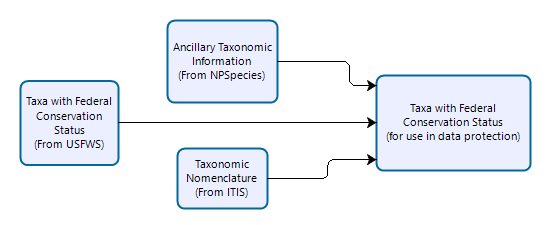
\includegraphics[width=7.64in]{vignettes/common/ProcessingWorkflow} \caption{Example general workflow to include in the methods section.}\label{fig:figure1}
\end{figure}

\hypertarget{data-collection-and-sample-processing-methods-optional}{%
\subsubsection{Data Collection and Sample Processing Methods
(optional)}\label{data-collection-and-sample-processing-methods-optional}}

Include a description of field methods and sample processing

\hypertarget{additional-data-sources-optional}{%
\subsubsection{Additional Data Sources
(optional)}\label{additional-data-sources-optional}}

Provide descriptions (with citations) of other data sources used.

\hypertarget{data-processing-required-if-done}{%
\subsubsection{Data Processing (required if
done)}\label{data-processing-required-if-done}}

Summarize process and results of any QC processes done that manipulate,
change, or qualify data.

\hypertarget{code-availability-required}{%
\subsubsection{Code Availability
(required)}\label{code-availability-required}}

For all studies using custom code in the generation or processing of
datasets, a statement must be included indicating whether and how the
code can be accessed and any restrictions to access. This section should
also include information on the versions of any software used, if
relevant, and any specific variables or parameters used to generate,
test, or process the current dataset. Actual analytical code should be
provided in Appendices.

\hypertarget{references-required}{%
\section{References (required)}\label{references-required}}

Provide sufficient information to locate the resource. If the citation
has a DOI, include the DOI at the end of the citation, including the
\url{https://doi.org} prefix. If you are citing documents that have
unregistered DOIs (such as a data package that you are working on
concurrently) still include the DOI. Electronic resources data and data
services or web sites should include the date they were accessed. Keep
the following line of code if you would like to automate generating and
formatting references:

\hypertarget{refs}{}
\begin{CSLReferences}{0}{0}
\end{CSLReferences}

If you would like to manually format your references, delete the
preceding two lines and use the following examples instead: Include
bibliographic information for any works cited (including the data
package the DRR is describing) in the above sections, using the standard
\emph{NPS NR Publication Series} referencing style.

See the following examples:

\hypertarget{agency-company-etc.-as-author-examples}{%
\subsubsection{Agency, Company, etc. as Author
Examples}\label{agency-company-etc.-as-author-examples}}

Fung Associates Inc.~and SWCA Environmental Consultants. 2010.
Assessment of natural resources and watershed conditions for Kalaupapa
National Historical Park. Natural Resource Report.
NPS/NPRC/WRD/NRR---2010/261. National Park Service, Fort Collins,
Colorado.

Greater Yellowstone Whitebark Pine Monitoring Working Group. 2014.
Monitoring whitebark pine in the Greater Yellowstone Ecosystem: 2013
annual report. Natural Resource Data Series. NPS/GRYN/NRDS---2014/631.
National Park Service. Fort Collins, Colorado.

National Park Service (NPS). 2016. State of the park report for Zion
National Park. State of the Park Reports. No.~23. National Park Service.
Washington, District of Columbia.

U.S. Forest Service (USFS). 1993. ECOMAP. National hierarchical
framework of ecological units. U. S. Forest Service, Washington, D.C.

\hypertarget{traditional-journal-article-examples}{%
\subsubsection{Traditional Journal Article
Examples}\label{traditional-journal-article-examples}}

Bradbury, J. W., S. L. Vehrencamp, K. E. Clifton, and L. M. Clifton.
1996. The relationship between bite rate and local forage abundance in
wild Thompson's gazelles. Ecology 77:2237--2255.
\url{https://doi.org/10.2307/2265717}

Oakley, K. L., L. P. Thomas, and S. G. Fancy. 2003. Guidelines for
long-term monitoring protocols. Wildlife Society Bulletin
31(4):1000--1003.

Sawaya, M. A., T. K. Ruth, S. Creel, J. J. Rotella, J. B. Stetz, H. B.
Quigley, and S. T. Kalinowski. 2011. Evaluation of noninvasive genetic
sampling methods for cougars in Yellowstone National Park. The Journal
of Wildlife Management 75(3):612--622.
\url{https://doi.org/10.1002/jwmg.92}

\hypertarget{book-example}{%
\subsubsection{Book Example}\label{book-example}}

Harvill, A. M., Jr., T. R. Bradley, C. E. Stevens, T. F. Wieboldt, D. M.
E. Ware, D. W. Ogle, and G. W. Ramsey. 1992. Atlas of the Virginia
flora, third edition. Virginia Botanical Associates, Farmville,
Virginia.

\hypertarget{book-chapter-examples}{%
\subsubsection{Book Chapter Examples}\label{book-chapter-examples}}

McCauly, E. 1984. The estimation of abundance and biomass of zooplankton
in samples. Pages 228--265 in J. A. Dowling and F. H. Rigler, editors. A
manual on methods for the assessment of secondary productivity in fresh
waters. Blackwell Scientific, Oxford, UK.

Watson, P. J. 2004. Of caves and shell mounds in west-central Kentucky.
Pages 159--164 in Of caves and shell mounds. The University of Alabama
Press, Tuscaloosa, Alabama.

\hypertarget{published-report-examples}{%
\subsubsection{Published Report
Examples}\label{published-report-examples}}

Bass, S., R. E. Gallipeau, Jr., M. Van Stappen, J. Kumer, M. Wessner, S.
Petersburg, L. L. Hays, J. Milstone, M. Soukup, M. Fletcher, L. G.
Adams, and others. 1988. Highlights of natural resource management 1987.
National Park Service, Denver, Colorado.

Holthausen, R. S., M. G. Raphael, K. S. McKelvey, E. D. Forsman, E. E.
Starkey, and D. E. Seaman. 1994. The contribution of federal and
nonfederal habitats to the persistence of the northern spotted owl on
the Olympic Peninsula, Washington. General Technical Report
PNW--GTR--352. U.S. Forest Service, Corvallis, Oregon.
\url{https://doi.org/10.2737/PNW-GTR-352}

Jackson, L. L., and L. P. Gough. 1991. Seasonal and spatial
biogeochemical trends for chaparral vegetation and soil geochemistry in
the Santa Monica Mountains National Recreation Area. U.S. Geological
Survey, Denver. Open File Report 91--0005.
\url{https://doi.org/10.3133/ofr915}

\hypertarget{unpublished-report-examples}{%
\subsubsection{Unpublished Report
Examples}\label{unpublished-report-examples}}

Conant, B., and J. I. Hodges. 1995. Western brant population estimates.
U.S. Fish and Wildlife Service Unpublished Report, Juneau, Alaska.

Conant, B., and J. F. Voelzer. 2001. Winter waterfowl survey: Mexico
west coast and Baja California. U.S. Fish and Wildlife Service
Unpublished Report, Juneau, Alaska.

\hypertarget{thesisdissertation-examples}{%
\subsubsection{Thesis/Dissertation
Examples}\label{thesisdissertation-examples}}

Diong, C. H. 1982. Population and biology of the feral pig (Sus scrofa
L) in Kipahulu Valley, Mau'i. Dissertation. University of Hawai'i,
Honolulu, Hawai'i.

McTigue, K. M. 1992. Nutrient pulses and herbivory: Integrative control
of primary producers in lakes. Thesis. University of Wisconsin, Madison,
Wisconsin.

\hypertarget{conference-proceedings-examples}{%
\subsubsection{Conference Proceedings
Examples}\label{conference-proceedings-examples}}

Gunther, K. A. 1994. Changing problems in bear management: Yellowstone
National Park twenty-plus years after the dumps. Ninth International
Conference on Bear Research and Management. Missoula, MT, International
Association for Bear Research and Management, Bozeman, Montana, February
1992:549--560.

Webb, J. R., and J. N. Galloway. 1991. Potential acidification of
streams in Mid-Appalachian Highlands: A problem with generalized
assessments. Southern Appalachian Man and Biosphere Conference.
Gatlinburg, Tennessee.

\hypertarget{general-internet-examples}{%
\subsubsection{General Internet
Examples}\label{general-internet-examples}}

Colorado Native Plant Society. 2016. Colorado Native Plant Society
website. Available at: \url{https://conps.org/} (accessed 07 March
2016).

National Park Service (NPS). 2016a. IRMA Portal (Integrated Resource
Management Applications) website. Available at:
\url{https://irma.nps.gov} (accessed 07 March 2016),

National Park Service (NPS). 2016b. Natural Resource Publications
Management website. Available at:
\url{http://www.nature.nps.gov/publications/nrpm/} (accessed 07 March
2016).

United Sates Fish and Wildlife Service (USFWS). 2016. Endangered Species
website. Available at: \url{http://www.fws.gov/endangered/} (accessed 07
March 2016).

\hypertarget{online-data-warehouse-sites-sites-that-allow-you-see-and-download-data-from-multiple-sources}{%
\subsubsection{Online Data Warehouse Sites (sites that allow you see and
download data from multiple
sources)}\label{online-data-warehouse-sites-sites-that-allow-you-see-and-download-data-from-multiple-sources}}

National Oceanographic and Atmospheric Association (NOAA). 2016. NOAA
National Climatic Data Center website. Available at:
\url{http://www.ncdc.noaa.gov/} (accessed 07 March 2016).

Environmental Protection Agency (EPA). 2016. Storage and Retrieval Data
Warehouse website (STORET). Available at:
\url{http://www.epa.gov/storet/} (accessed 07 March 2016).

National Park Service (NPS). 2016c. NPScape Landscape Dynamics Metric
Viewer website. Available at:
\url{http://science.nature.nps.gov/im/monitor/npscape/viewer/} (accessed
07 March 2016).

National Park Service (NPS). 2016d. NPSpecies online application.
Available at: \url{https://irma.nps.gov/NPSpecies/} (accessed 07 March
2016).

United States Geologic Survey (USGS). 2016. BioData - Aquatic
Bioassessment Data for the Nation. Available at:
\url{https://aquatic.biodata.usgs.gov/} (accessed 07 March 2016).

\hypertarget{acknowledgements-optional}{%
\section{Acknowledgements (optional)}\label{acknowledgements-optional}}

The Acknowledgements should contain text acknowledging non-author
contributors. Acknowledgements should be brief, and should not include
thanks to anonymous referees and editors or effusive comments. Grant or
contribution numbers may be acknowledged.

\hypertarget{appendix-a.-code-listing}{%
\section{Appendix A. Code Listing}\label{appendix-a.-code-listing}}

In most cases, Code listing is not required. If all QA/QC and data
manipulations were performed elsewhere, you should cite that code in the
methods (and leave the ``Listing'' code chunk as the default settings:
eval=FALSE and echo=FALSE). If you have developed custom scripts, you
can add those to DataStore with the reference type ``Script'' and cite
them in the DRR. Some people have developed code to perform QA/QC or
data manipulation within the DRR itself. In that case, you must set the
``Listing'' code chunk to eval=TRUE and echo=TRUE to fully document the
QA/QC process.

\begin{Shaded}
\begin{Highlighting}[]
\CommentTok{\# The title of your DRR. Should all DRR start with "Data Release Report:"? Should we enforce titles specifically referencing the data package(s) they the report is about?}
\NormalTok{title }\OtherTok{\textless{}{-}} \StringTok{"DRR Title"}

\CommentTok{\# Optional and should only be included if publishing to the semi{-}official DRR series. Contact Joe if you are. If not, leave as NULL}
\NormalTok{reportNumber }\OtherTok{\textless{}{-}} \StringTok{": get this number from Joe DeVivo"}

\CommentTok{\# This should match the Data Store Reference ID for this DRR. Eventually we should be able to pull this directly from the data package metadata.}
\NormalTok{DRR\_DSRefID }\OtherTok{\textless{}{-}} \DecValTok{7654321}

\CommentTok{\#Author names and affiliations:}

\CommentTok{\#One way to think of the author information is that you are building a table:}

\CommentTok{\# Author | Affiliation | ORCID}
\CommentTok{\# Jane   | Institute 1 | 0000{-}1111{-}2222{-}3333}
\CommentTok{\# Jane   | Institute 2 | 0000{-}1111{-}2222{-}3333}
\CommentTok{\# John   | Institute 2 | NA}

\CommentTok{\#once the table is built, authors can be associated with the appropriate institute via relevant superscripts and the institutes can be listed only once in the DRR.}

\CommentTok{\# list the authors. If an author has multiple institutional affiliations, you must list the author multiple times. In this example, Jane Doe is listed twice because she has two affiliations.}
\NormalTok{authorNames }\OtherTok{\textless{}{-}} \FunctionTok{c}\NormalTok{(}
  \StringTok{"Jane Doe"}\NormalTok{,}
  \StringTok{"Jane Doe"}\NormalTok{,}
  \StringTok{"John Doe"}
\NormalTok{)}

\CommentTok{\# List author affiliations. The order of author affiliations must match the order of the authors in AuthorNames. If an author has multiple affiliations, the author must be listed 2 (or more) times under authorNames (above) and each affiliation should be listed in order. If authors share the same affiliation, the affiliation should be listed once for each author. In this case, Managed Business Solutions (MBS) is listed twice because it is associated with two authors. MBS will only print to the DRR once.}

\CommentTok{\#Note that the entirety of each affiliation is enclosed in quotations. Do not worry about indentation or word wrapping.}
\NormalTok{authorAffiliations }\OtherTok{\textless{}{-}} \FunctionTok{c}\NormalTok{(}
  \StringTok{"NPS Inventory and Monitory Division, 1201 Oakridge Dr, Suite 150, Fort Collins, Colorado"}\NormalTok{, }
  \StringTok{"Managed Business Solutions (MBS), a Sealaska Company, Contractor to the National Park Service, Natural Resource Stewardship and Science Directorate, 1201 Oakridge Dr, Suite 150, Fort Collins, Colorado"}\NormalTok{,}
  \StringTok{"Managed Business Solutions (MBS), a Sealaska Company, Contractor to the National Park Service, Natural Resource Stewardship and Science Directorate, 1201 Oakridge Dr, Suite 150, Fort Collins, Colorado"}
\NormalTok{)}

\CommentTok{\# List the ORCID iDs for each author in the format "xxxx{-}xxxx{-}xxxx{-}xxxx". If an author does not have an ORCID iD, specify NA (no quotes). If an author is listed more than once (for instance because they have multiple institutional affiliations), the ORCID iD must also be listed more than once. For more information on ORCID iDs and to register an ORCID iD, see https://www.orcid.org. }

\CommentTok{\#The order of the ORCID iDs must match the order of authors in AuthorNames.In this example, Jane Doe has an ORCID iD but John Doe does not. Jane\textquotesingle{}s ORCID iD is listed twice because she her name is listed twice in authorNames(because she has two authorAffiliations).}
\NormalTok{authorORCID }\OtherTok{\textless{}{-}} \FunctionTok{c}\NormalTok{(}
  \StringTok{"0000{-}1111{-}2222{-}3333"}\NormalTok{, }\StringTok{"0000{-}1111{-}2222{-}3333"}\NormalTok{, }\ConstantTok{NA}
\NormalTok{  )}

\CommentTok{\# Replace the text below with your abstract.}
\NormalTok{DRRabstract }\OtherTok{\textless{}{-}} \StringTok{"Abstract Should go here. Multiple Lines are okay; it\textquotesingle{}ll format correctly. Pay careful attention to non{-}standard characters, line breaks (\textless{}br\textgreater{}), carriage returns, and curly{-}quotes. You may find it useful to write the abstract in NotePad++ or some other text editor and not a word processor (such as Microsoft Word).}\SpecialCharTok{\textbackslash{}n\textbackslash{}n}

\StringTok{Note that if you need multiple paragraphs or line breaks you can generate them using a combination of backslashes and n\textquotesingle{}s. }\SpecialCharTok{\textbackslash{}n\textbackslash{}n}

\StringTok{The abstract should succinctly describe the study, the assay(s) performed, the resulting data, and their reuse potential, but should not make any claims regarding new scientific findings. No references are allowed in this section."}

\CommentTok{\# DataStore reference ID for the data package associated with this report. You must have at least one data package.Eventually, we will automate importing much of this information from metadata.}
\NormalTok{dataPackageRefID }\OtherTok{\textless{}{-}} \FunctionTok{c}\NormalTok{(}\DecValTok{12342567}\NormalTok{)}

\CommentTok{\# Must match title in DataStore and metadata}
\NormalTok{dataPackageTitle }\OtherTok{\textless{}{-}} \StringTok{"Data Package Title"}

\CommentTok{\# Must match descriptions in the data package metadata}
\NormalTok{dataPackageDescription }\OtherTok{\textless{}{-}} \StringTok{"Short title for data package1"}

\CommentTok{\# generates your data package DOI based on the data package DataStore reference ID. This is different from the DRR DOI! No need to edit this.}
\NormalTok{dataPackageDOI }\OtherTok{\textless{}{-}} \FunctionTok{paste0}\NormalTok{(}\StringTok{"https://doi.org/10.57830/"}\NormalTok{, dataPackageRefID)}

\CommentTok{\# list the file names in your data package. Do NOT include metadata files.}
\NormalTok{dataPackage\_fileNames }\OtherTok{\textless{}{-}} \FunctionTok{c}\NormalTok{(}
  \StringTok{"my\_data.csv"}\NormalTok{,}
  \StringTok{"my\_data2.csv"}
\NormalTok{)}

\CommentTok{\# list the approximate size of each data file. Make sure the order corresponds to the order of of the file names in dataPackage\_fileNames}
\NormalTok{dataPackage\_fileSizes }\OtherTok{\textless{}{-}} \FunctionTok{c}\NormalTok{(}\StringTok{"0.8 MB"}\NormalTok{, }\StringTok{"10 GB"}\NormalTok{)}

\CommentTok{\# list a short, one{-}line description of each data file. Descriptions must be in the same order as the filenames.}
\NormalTok{dataPackage\_fileDescript }\OtherTok{\textless{}{-}} \FunctionTok{c}\NormalTok{(}
  \StringTok{"This is a short description of my\_data.csv (a good guideline is 10 words or less)."}\NormalTok{,}
  \StringTok{"This is a short description of my\_data2.csv."}\NormalTok{)}
\NormalTok{RRpackages }\OtherTok{\textless{}{-}} \FunctionTok{c}\NormalTok{(}\StringTok{"markdown"}\NormalTok{,}
                \StringTok{"rmarkdown"}\NormalTok{,}
                \StringTok{"pander"}\NormalTok{,}
                \StringTok{"knitr"}\NormalTok{,}
                \StringTok{"yaml"}\NormalTok{,}
                \StringTok{"kableExtra"}\NormalTok{,}
                \StringTok{"devtools"}\NormalTok{,}
                \StringTok{"tidyverse"}\NormalTok{)}

\NormalTok{inst }\OtherTok{\textless{}{-}}\NormalTok{ RRpackages }\SpecialCharTok{\%in\%} \FunctionTok{installed.packages}\NormalTok{()}
\ControlFlowTok{if}\NormalTok{ (}\FunctionTok{length}\NormalTok{(RRpackages[}\SpecialCharTok{!}\NormalTok{inst]) }\SpecialCharTok{\textgreater{}} \DecValTok{0}\NormalTok{) \{}
  \FunctionTok{install.packages}\NormalTok{(RRpackages[}\SpecialCharTok{!}\NormalTok{inst], }\AttributeTok{dep =} \ConstantTok{TRUE}\NormalTok{, }\AttributeTok{repos =} \StringTok{"https://cloud.r{-}project.org"}\NormalTok{)}
\NormalTok{\}}
\FunctionTok{lapply}\NormalTok{(RRpackages, library, }\AttributeTok{character.only =} \ConstantTok{TRUE}\NormalTok{)}
\end{Highlighting}
\end{Shaded}

\begin{verbatim}
## [[1]]
##  [1] "QCkit"      "lubridate"  "forcats"    "stringr"    "dplyr"     
##  [6] "purrr"      "readr"      "tidyr"      "tibble"     "ggplot2"   
## [11] "tidyverse"  "devtools"   "usethis"    "kableExtra" "yaml"      
## [16] "knitr"      "pander"     "rmarkdown"  "markdown"   "stats"     
## [21] "graphics"   "grDevices"  "utils"      "datasets"   "methods"   
## [26] "base"      
## 
## [[2]]
##  [1] "QCkit"      "lubridate"  "forcats"    "stringr"    "dplyr"     
##  [6] "purrr"      "readr"      "tidyr"      "tibble"     "ggplot2"   
## [11] "tidyverse"  "devtools"   "usethis"    "kableExtra" "yaml"      
## [16] "knitr"      "pander"     "rmarkdown"  "markdown"   "stats"     
## [21] "graphics"   "grDevices"  "utils"      "datasets"   "methods"   
## [26] "base"      
## 
## [[3]]
##  [1] "QCkit"      "lubridate"  "forcats"    "stringr"    "dplyr"     
##  [6] "purrr"      "readr"      "tidyr"      "tibble"     "ggplot2"   
## [11] "tidyverse"  "devtools"   "usethis"    "kableExtra" "yaml"      
## [16] "knitr"      "pander"     "rmarkdown"  "markdown"   "stats"     
## [21] "graphics"   "grDevices"  "utils"      "datasets"   "methods"   
## [26] "base"      
## 
## [[4]]
##  [1] "QCkit"      "lubridate"  "forcats"    "stringr"    "dplyr"     
##  [6] "purrr"      "readr"      "tidyr"      "tibble"     "ggplot2"   
## [11] "tidyverse"  "devtools"   "usethis"    "kableExtra" "yaml"      
## [16] "knitr"      "pander"     "rmarkdown"  "markdown"   "stats"     
## [21] "graphics"   "grDevices"  "utils"      "datasets"   "methods"   
## [26] "base"      
## 
## [[5]]
##  [1] "QCkit"      "lubridate"  "forcats"    "stringr"    "dplyr"     
##  [6] "purrr"      "readr"      "tidyr"      "tibble"     "ggplot2"   
## [11] "tidyverse"  "devtools"   "usethis"    "kableExtra" "yaml"      
## [16] "knitr"      "pander"     "rmarkdown"  "markdown"   "stats"     
## [21] "graphics"   "grDevices"  "utils"      "datasets"   "methods"   
## [26] "base"      
## 
## [[6]]
##  [1] "QCkit"      "lubridate"  "forcats"    "stringr"    "dplyr"     
##  [6] "purrr"      "readr"      "tidyr"      "tibble"     "ggplot2"   
## [11] "tidyverse"  "devtools"   "usethis"    "kableExtra" "yaml"      
## [16] "knitr"      "pander"     "rmarkdown"  "markdown"   "stats"     
## [21] "graphics"   "grDevices"  "utils"      "datasets"   "methods"   
## [26] "base"      
## 
## [[7]]
##  [1] "QCkit"      "lubridate"  "forcats"    "stringr"    "dplyr"     
##  [6] "purrr"      "readr"      "tidyr"      "tibble"     "ggplot2"   
## [11] "tidyverse"  "devtools"   "usethis"    "kableExtra" "yaml"      
## [16] "knitr"      "pander"     "rmarkdown"  "markdown"   "stats"     
## [21] "graphics"   "grDevices"  "utils"      "datasets"   "methods"   
## [26] "base"      
## 
## [[8]]
##  [1] "QCkit"      "lubridate"  "forcats"    "stringr"    "dplyr"     
##  [6] "purrr"      "readr"      "tidyr"      "tibble"     "ggplot2"   
## [11] "tidyverse"  "devtools"   "usethis"    "kableExtra" "yaml"      
## [16] "knitr"      "pander"     "rmarkdown"  "markdown"   "stats"     
## [21] "graphics"   "grDevices"  "utils"      "datasets"   "methods"   
## [26] "base"
\end{verbatim}

\begin{Shaded}
\begin{Highlighting}[]
\NormalTok{devtools}\SpecialCharTok{::}\FunctionTok{install\_github}\NormalTok{(}\StringTok{"nationalparkservice/QCkit"}\NormalTok{)}
\end{Highlighting}
\end{Shaded}

\begin{verbatim}
## Skipping install of 'QCkit' from a github remote, the SHA1 (930652d3) has not changed since last install.
##   Use `force = TRUE` to force installation
\end{verbatim}

\begin{Shaded}
\begin{Highlighting}[]
\FunctionTok{library}\NormalTok{(QCkit)}
\NormalTok{date }\OtherTok{\textless{}{-}} \FunctionTok{format}\NormalTok{(}\FunctionTok{Sys.time}\NormalTok{(), }\StringTok{"\%d \%B, \%Y"}\NormalTok{)}
\FunctionTok{cat}\NormalTok{(}\StringTok{"\#"}\NormalTok{, title, }\StringTok{"}\SpecialCharTok{\textbackslash{}n}\StringTok{"}\NormalTok{)}
\end{Highlighting}
\end{Shaded}

\begin{verbatim}
## # DRR Title
\end{verbatim}

\begin{Shaded}
\begin{Highlighting}[]
\ControlFlowTok{if}\NormalTok{ (}\SpecialCharTok{!}\FunctionTok{is.null}\NormalTok{(reportNumber)) \{}
\NormalTok{  subtitle }\OtherTok{\textless{}{-}} \FunctionTok{paste0}\NormalTok{(}\StringTok{"Data Release Report "}\NormalTok{, reportNumber)}
  \FunctionTok{cat}\NormalTok{(}\StringTok{"\#\#\#"}\NormalTok{, subtitle)}
\NormalTok{\}}
\end{Highlighting}
\end{Shaded}

\begin{verbatim}
## ### Data Release Report : get this number from Joe DeVivo
\end{verbatim}

\begin{Shaded}
\begin{Highlighting}[]
\NormalTok{author\_list }\OtherTok{\textless{}{-}} \FunctionTok{data.frame}\NormalTok{(authorNames, authorAffiliations, authorORCID)}
\NormalTok{unique\_authors }\OtherTok{\textless{}{-}}\NormalTok{ author\_list }\SpecialCharTok{\%\textgreater{}\%} \FunctionTok{distinct}\NormalTok{(authorNames,}
                                           \AttributeTok{.keep\_all =} \ConstantTok{TRUE}\NormalTok{)}
\NormalTok{unique\_affiliation }\OtherTok{\textless{}{-}}\NormalTok{ author\_list }\SpecialCharTok{\%\textgreater{}\%} \FunctionTok{distinct}\NormalTok{(authorAffiliations,}
                                              \AttributeTok{.keep\_all =} \ConstantTok{TRUE}\NormalTok{)}

\CommentTok{\#single author documents:}
\ControlFlowTok{if}\NormalTok{(}\FunctionTok{length}\NormalTok{(}\FunctionTok{seq\_along}\NormalTok{(unique\_authors}\SpecialCharTok{$}\NormalTok{authorNames)) }\SpecialCharTok{==} \DecValTok{1}\NormalTok{)\{}

  \ControlFlowTok{for}\NormalTok{ (i }\ControlFlowTok{in} \FunctionTok{seq\_along}\NormalTok{(unique\_authors}\SpecialCharTok{$}\NormalTok{authorNames)) \{}
\NormalTok{    curr }\OtherTok{\textless{}{-}}\NormalTok{ unique\_authors[i, ]}
    
    \CommentTok{\#find all author affiliations}
\NormalTok{    aff }\OtherTok{\textless{}{-}}\NormalTok{ author\_list[}\FunctionTok{which}\NormalTok{(authorNames }\SpecialCharTok{==}\NormalTok{ curr}\SpecialCharTok{$}\NormalTok{authorNames),]}
\NormalTok{    aff }\OtherTok{\textless{}{-}}\NormalTok{ aff}\SpecialCharTok{$}\NormalTok{authorAffiliations  }
    
    \CommentTok{\#identify order of affiliation(s) in a unique list of affiliations}
    \CommentTok{\#build the superscripts for author affiliations}
\NormalTok{    super\_script }\OtherTok{\textless{}{-}}\NormalTok{ unique\_affiliation}\SpecialCharTok{$}\NormalTok{authorAffiliations }\SpecialCharTok{\%in\%}\NormalTok{ aff }
\NormalTok{    super }\OtherTok{\textless{}{-}} \FunctionTok{which}\NormalTok{(super\_script }\SpecialCharTok{==} \ConstantTok{TRUE}\NormalTok{)}
\NormalTok{    script }\OtherTok{\textless{}{-}}\NormalTok{ super}
    
    \ControlFlowTok{if}\NormalTok{(}\FunctionTok{length}\NormalTok{(}\FunctionTok{seq\_along}\NormalTok{(super)) }\SpecialCharTok{\textgreater{}} \DecValTok{1}\NormalTok{)\{}
\NormalTok{      script }\OtherTok{\textless{}{-}} \ConstantTok{NULL}
\NormalTok{      j }\OtherTok{\textless{}{-}} \DecValTok{1}
      \ControlFlowTok{while}\NormalTok{(j }\SpecialCharTok{\textless{}} \FunctionTok{length}\NormalTok{(}\FunctionTok{seq\_along}\NormalTok{(super)))\{}
\NormalTok{        script }\OtherTok{\textless{}{-}} \FunctionTok{append}\NormalTok{(script, }\FunctionTok{paste0}\NormalTok{(super[j],}\StringTok{","}\NormalTok{))}
\NormalTok{        j }\OtherTok{\textless{}{-}}\NormalTok{ j}\SpecialCharTok{+}\DecValTok{1}
\NormalTok{      \}}
      \ControlFlowTok{if}\NormalTok{(j }\SpecialCharTok{==} \FunctionTok{length}\NormalTok{(}\FunctionTok{seq\_along}\NormalTok{(super)))\{}
\NormalTok{        script }\OtherTok{\textless{}{-}} \FunctionTok{append}\NormalTok{(script, super[j])}
\NormalTok{      \}}
\NormalTok{    \}}
\NormalTok{  \}}
   \FunctionTok{cat}\NormalTok{(}\StringTok{"\#\#\#\# "}\NormalTok{, curr}\SpecialCharTok{$}\NormalTok{authorNames, }\StringTok{","}\NormalTok{, }\StringTok{"\^{}"}\NormalTok{,script,}\StringTok{"\^{}"}\NormalTok{, }\StringTok{" "}\NormalTok{, }\StringTok{" "}\NormalTok{, }\AttributeTok{sep=}\StringTok{""}\NormalTok{)}
        \ControlFlowTok{if}\NormalTok{ (}\FunctionTok{is.na}\NormalTok{(curr}\SpecialCharTok{$}\NormalTok{authorORCID)) \{}
\NormalTok{        \}}
        \ControlFlowTok{if}\NormalTok{ (}\SpecialCharTok{!}\FunctionTok{is.na}\NormalTok{(curr}\SpecialCharTok{$}\NormalTok{authorORCID)) \{}
\NormalTok{          orc }\OtherTok{\textless{}{-}} \FunctionTok{paste0}\NormalTok{(}\StringTok{"https://orcid.org/"}\NormalTok{, curr}\SpecialCharTok{$}\NormalTok{authorORCID, }\StringTok{" "}\NormalTok{)}
          \FunctionTok{cat}\NormalTok{(\{\{ orc \}\})}
\NormalTok{        \}}
  
  \CommentTok{\#cat("\#\#\#\# ", unique\_authors$authorNames, "\^{}1\^{}", sep="")}
  \CommentTok{\#if(!is.na(authorORCID))\{}
  \CommentTok{\#  orc \textless{}{-} paste0(" https://orcid.org/", unique\_authors$authorORCID)}
  \CommentTok{\#  cat(\{\{ orc \}\}, "\textbackslash{}n")}
  \CommentTok{\#\}}
  \CommentTok{\#cat("\#\#\#\# ", unique\_authors$authorAffiliations, sep="")}
\NormalTok{\}}
  
\CommentTok{\#multi author documents:}
\ControlFlowTok{if}\NormalTok{(}\FunctionTok{length}\NormalTok{(}\FunctionTok{seq\_along}\NormalTok{(unique\_authors}\SpecialCharTok{$}\NormalTok{authorNames)) }\SpecialCharTok{\textgreater{}} \DecValTok{1}\NormalTok{)\{}
  \ControlFlowTok{for}\NormalTok{ (i }\ControlFlowTok{in} \FunctionTok{seq\_along}\NormalTok{(unique\_authors}\SpecialCharTok{$}\NormalTok{authorNames)) \{}
\NormalTok{    curr }\OtherTok{\textless{}{-}}\NormalTok{ unique\_authors[i, ]}
    
    \CommentTok{\#find all author affiliations}
\NormalTok{    aff }\OtherTok{\textless{}{-}}\NormalTok{ author\_list[}\FunctionTok{which}\NormalTok{(authorNames }\SpecialCharTok{==}\NormalTok{ curr}\SpecialCharTok{$}\NormalTok{authorNames),]}
\NormalTok{    aff }\OtherTok{\textless{}{-}}\NormalTok{ aff}\SpecialCharTok{$}\NormalTok{authorAffiliations  }
    
    \CommentTok{\#identify order of affiliation(s) in a unique list of affiliations}
    \CommentTok{\#build the superscripts for author affiliations}
\NormalTok{    super\_script }\OtherTok{\textless{}{-}}\NormalTok{ unique\_affiliation}\SpecialCharTok{$}\NormalTok{authorAffiliations }\SpecialCharTok{\%in\%}\NormalTok{ aff }
\NormalTok{    super }\OtherTok{\textless{}{-}} \FunctionTok{which}\NormalTok{(super\_script }\SpecialCharTok{==} \ConstantTok{TRUE}\NormalTok{)}
\NormalTok{    script }\OtherTok{\textless{}{-}}\NormalTok{ super}
    
    \ControlFlowTok{if}\NormalTok{(}\FunctionTok{length}\NormalTok{(}\FunctionTok{seq\_along}\NormalTok{(super)) }\SpecialCharTok{\textgreater{}} \DecValTok{1}\NormalTok{)\{}
\NormalTok{      script }\OtherTok{\textless{}{-}} \ConstantTok{NULL}
\NormalTok{      j }\OtherTok{\textless{}{-}} \DecValTok{1}
      \ControlFlowTok{while}\NormalTok{(j }\SpecialCharTok{\textless{}} \FunctionTok{length}\NormalTok{(}\FunctionTok{seq\_along}\NormalTok{(super)))\{}
\NormalTok{        script }\OtherTok{\textless{}{-}} \FunctionTok{append}\NormalTok{(script, }\FunctionTok{paste0}\NormalTok{(super[j],}\StringTok{","}\NormalTok{))}
\NormalTok{        j }\OtherTok{\textless{}{-}}\NormalTok{ j}\SpecialCharTok{+}\DecValTok{1}
\NormalTok{      \}}
      \ControlFlowTok{if}\NormalTok{(j }\SpecialCharTok{==} \FunctionTok{length}\NormalTok{(}\FunctionTok{seq\_along}\NormalTok{(super)))\{}
\NormalTok{        script }\OtherTok{\textless{}{-}} \FunctionTok{append}\NormalTok{(script, super[j])}
\NormalTok{      \}}
\NormalTok{    \}}
    
    \CommentTok{\# if NOT the second{-}to{-}last author:}
    \ControlFlowTok{if}\NormalTok{(i }\SpecialCharTok{\textless{}}\NormalTok{ (}\FunctionTok{length}\NormalTok{(}\FunctionTok{seq\_along}\NormalTok{(unique\_authors}\SpecialCharTok{$}\NormalTok{authorNames)) }\SpecialCharTok{{-}} \DecValTok{1}\NormalTok{))\{}
      \FunctionTok{cat}\NormalTok{(}\StringTok{"\#\#\#\# "}\NormalTok{, curr}\SpecialCharTok{$}\NormalTok{authorNames, }\StringTok{","}\NormalTok{, }\StringTok{"\^{}"}\NormalTok{,script,}\StringTok{"\^{}"}\NormalTok{, }\StringTok{" "}\NormalTok{, }\StringTok{" "}\NormalTok{, }\AttributeTok{sep=}\StringTok{""}\NormalTok{)}
        \ControlFlowTok{if}\NormalTok{ (}\FunctionTok{is.na}\NormalTok{(curr}\SpecialCharTok{$}\NormalTok{authorORCID)) \{}
\NormalTok{        \}}
        \ControlFlowTok{if}\NormalTok{ (}\SpecialCharTok{!}\FunctionTok{is.na}\NormalTok{(curr}\SpecialCharTok{$}\NormalTok{authorORCID)) \{}
\NormalTok{          orc }\OtherTok{\textless{}{-}} \FunctionTok{paste0}\NormalTok{(}\StringTok{"https://orcid.org/"}\NormalTok{, curr}\SpecialCharTok{$}\NormalTok{authorORCID, }\StringTok{" "}\NormalTok{)}
          \FunctionTok{cat}\NormalTok{(\{\{ orc \}\})}
\NormalTok{        \}}
\NormalTok{    \}}
    
    \CommentTok{\# if IS the second{-}to{-}last author}
    \ControlFlowTok{if}\NormalTok{(i }\SpecialCharTok{==}\NormalTok{ (}\FunctionTok{length}\NormalTok{(}\FunctionTok{seq\_along}\NormalTok{(unique\_authors}\SpecialCharTok{$}\NormalTok{authorNames)) }\SpecialCharTok{{-}} \DecValTok{1}\NormalTok{))\{ }
       
      \CommentTok{\#if 3 or more authors, include a comma before the "and":}
      \ControlFlowTok{if}\NormalTok{(}\FunctionTok{length}\NormalTok{(}\FunctionTok{seq\_along}\NormalTok{(unique\_authors}\SpecialCharTok{$}\NormalTok{authorNames)) }\SpecialCharTok{\textgreater{}} \DecValTok{2}\NormalTok{)\{}
        \FunctionTok{cat}\NormalTok{(curr}\SpecialCharTok{$}\NormalTok{authorNames, }\StringTok{","}\NormalTok{,}\StringTok{"\^{}"}\NormalTok{,script,}\StringTok{"\^{} "}\NormalTok{, }\AttributeTok{sep=}\StringTok{""}\NormalTok{)}
        \ControlFlowTok{if}\NormalTok{ (}\FunctionTok{is.na}\NormalTok{(curr}\SpecialCharTok{$}\NormalTok{authorORCID)) \{}
\NormalTok{        \}}
        \ControlFlowTok{if}\NormalTok{ (}\SpecialCharTok{!}\FunctionTok{is.na}\NormalTok{(curr}\SpecialCharTok{$}\NormalTok{authorORCID)) \{}
\NormalTok{          orc }\OtherTok{\textless{}{-}} \FunctionTok{paste0}\NormalTok{(}\StringTok{"https://orcid.org/"}\NormalTok{, curr}\SpecialCharTok{$}\NormalTok{authorORCID, }\StringTok{" "}\NormalTok{)}
          \FunctionTok{cat}\NormalTok{(\{\{ orc \}\})}
\NormalTok{        \}}
        \FunctionTok{cat}\NormalTok{(}\StringTok{"and "}\NormalTok{, }\AttributeTok{sep=}\StringTok{""}\NormalTok{)}
\NormalTok{      \}}
      
      \CommentTok{\#If only 2 authors, omit comma before "and":}
      \ControlFlowTok{if}\NormalTok{(}\FunctionTok{length}\NormalTok{(}\FunctionTok{seq\_along}\NormalTok{(unique\_authors}\SpecialCharTok{$}\NormalTok{authorNames)) }\SpecialCharTok{==} \DecValTok{2}\NormalTok{)\{}
        \FunctionTok{cat}\NormalTok{(}\StringTok{"\#\#\#\# "}\NormalTok{, curr}\SpecialCharTok{$}\NormalTok{authorNames, }\StringTok{"\^{}"}\NormalTok{,script,}\StringTok{"\^{} "}\NormalTok{, }\AttributeTok{sep=}\StringTok{""}\NormalTok{)}
        \ControlFlowTok{if}\NormalTok{ (}\FunctionTok{is.na}\NormalTok{(curr}\SpecialCharTok{$}\NormalTok{authorORCID)) \{}
\NormalTok{        \}}
        \ControlFlowTok{if}\NormalTok{ (}\SpecialCharTok{!}\FunctionTok{is.na}\NormalTok{(curr}\SpecialCharTok{$}\NormalTok{authorORCID)) \{}
\NormalTok{          orc }\OtherTok{\textless{}{-}} \FunctionTok{paste0}\NormalTok{(}\StringTok{"https://orcid.org/"}\NormalTok{, curr}\SpecialCharTok{$}\NormalTok{authorORCID, }\StringTok{" "}\NormalTok{)}
          \FunctionTok{cat}\NormalTok{(\{\{ orc \}\})}
\NormalTok{        \}}
        \FunctionTok{cat}\NormalTok{(}\StringTok{"and "}\NormalTok{, }\AttributeTok{sep=}\StringTok{""}\NormalTok{)}
\NormalTok{      \}}
\NormalTok{    \}}
    
    \CommentTok{\# if IS the Last author :}
    \ControlFlowTok{if}\NormalTok{(i }\SpecialCharTok{==} \FunctionTok{length}\NormalTok{(}\FunctionTok{seq\_along}\NormalTok{(unique\_authors}\SpecialCharTok{$}\NormalTok{authorNames)))\{}
      \FunctionTok{cat}\NormalTok{(curr}\SpecialCharTok{$}\NormalTok{authorNames, }\StringTok{"\^{}"}\NormalTok{, script, }\StringTok{"\^{}"}\NormalTok{, }\AttributeTok{sep=}\StringTok{""}\NormalTok{)}
        \ControlFlowTok{if}\NormalTok{ (}\FunctionTok{is.na}\NormalTok{(curr}\SpecialCharTok{$}\NormalTok{authorORCID)) \{}
\NormalTok{        \}}
        \ControlFlowTok{if}\NormalTok{ (}\SpecialCharTok{!}\FunctionTok{is.na}\NormalTok{(curr}\SpecialCharTok{$}\NormalTok{authorORCID)) \{}
\NormalTok{          orc }\OtherTok{\textless{}{-}} \FunctionTok{paste0}\NormalTok{(}\StringTok{" https://orcid.org/"}\NormalTok{, curr}\SpecialCharTok{$}\NormalTok{authorORCID, }\StringTok{" "}\NormalTok{)}
          \FunctionTok{cat}\NormalTok{(\{\{ orc \}\})}
\NormalTok{        \}}
\NormalTok{    \}}
\NormalTok{  \}}
\NormalTok{\}}
\end{Highlighting}
\end{Shaded}

\begin{verbatim}
## #### Jane Doe^1,2^ https://orcid.org/0000-1111-2222-3333 and John Doe^2^
\end{verbatim}

\begin{Shaded}
\begin{Highlighting}[]
\FunctionTok{cat}\NormalTok{(}\StringTok{"}\SpecialCharTok{\textbackslash{}n\textbackslash{}n}\StringTok{"}\NormalTok{)}
\end{Highlighting}
\end{Shaded}

\begin{Shaded}
\begin{Highlighting}[]
\ControlFlowTok{for}\NormalTok{(i }\ControlFlowTok{in} \DecValTok{1}\SpecialCharTok{:}\FunctionTok{nrow}\NormalTok{(unique\_affiliation))\{}
  \FunctionTok{cat}\NormalTok{(}\StringTok{"\^{}"}\NormalTok{,i,}\StringTok{"\^{} "}\NormalTok{, unique\_affiliation[i,}\DecValTok{2}\NormalTok{], }\StringTok{"}\SpecialCharTok{\textbackslash{}n\textbackslash{}n}\StringTok{"}\NormalTok{, }\AttributeTok{sep=}\StringTok{""}\NormalTok{)}
\NormalTok{  \}}
\end{Highlighting}
\end{Shaded}

\begin{verbatim}
## ^1^ NPS Inventory and Monitory Division, 1201 Oakridge Dr, Suite 150, Fort Collins, Colorado
## 
## ^2^ Managed Business Solutions (MBS), a Sealaska Company, Contractor to the National Park Service, Natural Resource Stewardship and Science Directorate, 1201 Oakridge Dr, Suite 150, Fort Collins, Colorado
\end{verbatim}

\begin{Shaded}
\begin{Highlighting}[]
\NormalTok{filelist }\OtherTok{\textless{}{-}} \FunctionTok{data.frame}\NormalTok{(dataPackage\_fileNames, dataPackage\_fileSizes, dataPackage\_fileDescript)}

\NormalTok{knitr}\SpecialCharTok{::}\FunctionTok{kable}\NormalTok{(filelist, }\AttributeTok{caption =} \FunctionTok{paste0}\NormalTok{(}\StringTok{"**Table 1: "}\NormalTok{, dataPackageTitle, }\StringTok{": List of data files**"}\NormalTok{), }\AttributeTok{col.names =} \FunctionTok{c}\NormalTok{(}\StringTok{"File Name"}\NormalTok{, }\StringTok{"Size"}\NormalTok{, }\StringTok{"Description"}\NormalTok{), }\AttributeTok{format =} \StringTok{"pandoc"}\NormalTok{)}
\end{Highlighting}
\end{Shaded}

\begin{longtable}[]{@{}lll@{}}
\caption{\textbf{Table 1: Data Package Title: List of data
files}}\tabularnewline
\toprule\noalign{}
File Name & Size & Description \\
\midrule\noalign{}
\endfirsthead
\toprule\noalign{}
File Name & Size & Description \\
\midrule\noalign{}
\endhead
\bottomrule\noalign{}
\endlastfoot
my\_data.csv & 0.8 MB & This is a short description of my\_data.csv (a
good guideline is 10 words or less). \\
my\_data2.csv & 10 GB & This is a short description of my\_data2.csv. \\
\end{longtable}

\begin{Shaded}
\begin{Highlighting}[]
\CommentTok{\#Generates a table with definitions for the data flags, A, AE, P, or R. Honestly not super useful and can probably be turned off (set eval=FALSE) if these are defined elsewhere in text.}
\NormalTok{flags}\OtherTok{\textless{}{-}}\FunctionTok{c}\NormalTok{(}\StringTok{"A"}\NormalTok{,}\StringTok{" "}\NormalTok{, }\StringTok{"AE"}\NormalTok{, }\StringTok{"P"}\NormalTok{, }\StringTok{"R"}\NormalTok{, }\StringTok{"NA"}\NormalTok{)}
\NormalTok{def}\OtherTok{\textless{}{-}}\FunctionTok{c}\NormalTok{(}\StringTok{"Accepted"}\NormalTok{,}\StringTok{" "}\NormalTok{, }\StringTok{"Accepted, estimated"}\NormalTok{, }\StringTok{"Provisional"}\NormalTok{, }\StringTok{"Rejected"}\NormalTok{, }\StringTok{"Missing"}\NormalTok{)}
\NormalTok{app}\OtherTok{\textless{}{-}}\FunctionTok{c}\NormalTok{(}\StringTok{"columns ending }\SpecialCharTok{\textbackslash{}"}\StringTok{\_flag}\SpecialCharTok{\textbackslash{}"}\StringTok{"}\NormalTok{, }\StringTok{"unflagged data"}\NormalTok{, }
       \FunctionTok{rep}\NormalTok{(}\StringTok{"columns ending }\SpecialCharTok{\textbackslash{}"}\StringTok{\_flag}\SpecialCharTok{\textbackslash{}"}\StringTok{"}\NormalTok{, }\DecValTok{3}\NormalTok{), }\StringTok{"All data"}\NormalTok{)}
\NormalTok{data\_flags}\OtherTok{\textless{}{-}}\FunctionTok{data.frame}\NormalTok{(flags, def, app)}

\NormalTok{knitr}\SpecialCharTok{::}\FunctionTok{kable}\NormalTok{(data\_flags, }\AttributeTok{caption =} \StringTok{"**Table 2: Description of data quality flags**"}\NormalTok{, }\AttributeTok{col.names=}\FunctionTok{c}\NormalTok{(}\StringTok{"Flag"}\NormalTok{, }\StringTok{"Definition"}\NormalTok{, }\StringTok{"Usage"}\NormalTok{), }\AttributeTok{format=}\StringTok{"pandoc"}\NormalTok{)}
\end{Highlighting}
\end{Shaded}

\begin{longtable}[]{@{}lll@{}}
\caption{\textbf{Table 2: Description of data quality
flags}}\tabularnewline
\toprule\noalign{}
Flag & Definition & Usage \\
\midrule\noalign{}
\endfirsthead
\toprule\noalign{}
Flag & Definition & Usage \\
\midrule\noalign{}
\endhead
\bottomrule\noalign{}
\endlastfoot
A & Accepted & columns ending ``\_flag'' \\
& & unflagged data \\
AE & Accepted, estimated & columns ending ``\_flag'' \\
P & Provisional & columns ending ``\_flag'' \\
R & Rejected & columns ending ``\_flag'' \\
NA & Missing & All data \\
\end{longtable}

\begin{Shaded}
\begin{Highlighting}[]
\CommentTok{\# To turn off, set eval=FALSE.}
\CommentTok{\# Generates a table with a single row summarizing data quality across all flagged columns of the entire data package. To add additional non{-}flagged columns, specify them with column names: cols=("my\_unflagged\_data1", "my\_unflagged\_data2)" or column numbers: cols=c(1:4). All non{-}missing data in unflagged columns is assumed accepted. }

\CommentTok{\#if your package is not in your working directory, you need to specify the directory:}
\NormalTok{path}\OtherTok{\textless{}{-}}\StringTok{"../../DataPackageWorkflow/dataPackages/BICY\_Veg\_Data\_Package\_Example"}
\NormalTok{dp\_flags }\OtherTok{\textless{}{-}}\NormalTok{ QCkit}\SpecialCharTok{::}\FunctionTok{get\_custom\_flags}\NormalTok{(}\AttributeTok{directory =}\NormalTok{ path, }\AttributeTok{output=}\StringTok{"package"}\NormalTok{)}

\CommentTok{\#generate table:}
\NormalTok{kableExtra}\SpecialCharTok{::}\FunctionTok{kbl}\NormalTok{(dp\_flags, }\AttributeTok{caption =} \StringTok{\textquotesingle{}**Table 3.1: Summary of data quality flags for the data package**\textquotesingle{}}\NormalTok{, }\AttributeTok{col.names =} \FunctionTok{c}\NormalTok{(}\StringTok{"A"}\NormalTok{, }\StringTok{"AE"}\NormalTok{, }\StringTok{"P"}\NormalTok{, }\StringTok{"R"}\NormalTok{, }\StringTok{"\% Missing (Mean)"}\NormalTok{, }\StringTok{"RRU (Mean)"}\NormalTok{, }\StringTok{"RRU (SD)"}\NormalTok{), }\AttributeTok{format =} \StringTok{"pandoc"}\NormalTok{, }\AttributeTok{digits=}\DecValTok{2}\NormalTok{)}
\end{Highlighting}
\end{Shaded}

\begin{longtable}[]{@{}rrrrrrr@{}}
\caption{\textbf{Table 3.1: Summary of data quality flags for the data
package}}\tabularnewline
\toprule\noalign{}
A & AE & P & R & \% Missing (Mean) & RRU (Mean) & RRU (SD) \\
\midrule\noalign{}
\endfirsthead
\toprule\noalign{}
A & AE & P & R & \% Missing (Mean) & RRU (Mean) & RRU (SD) \\
\midrule\noalign{}
\endhead
\bottomrule\noalign{}
\endlastfoot
2968 & 0 & 0 & 32 & 0 & 0.99 & 0.03 \\
\end{longtable}

\begin{Shaded}
\begin{Highlighting}[]
\CommentTok{\# To turn off, set eval=FALSE.}
\CommentTok{\# Generates a table summarizing data quality across all flagged columns of each data file. To add additional non{-}flagged columns, specify them with column names: cols=("my\_unflagged\_data1", "my\_unflagged\_data2)" or numbers: cols=c(1:4). All non{-}missing data in unflagged columns is assumed accepted. If a file has no flagged columns and no specified custom columns, all values for that data file will be listed as "NA".}

\CommentTok{\#set directory to the location of your data package}
\NormalTok{path}\OtherTok{\textless{}{-}}\StringTok{"../../DataPackageWorkflow/dataPackages/BICY\_Veg\_Data\_Package\_Example"}
\NormalTok{df\_flags }\OtherTok{\textless{}{-}}\NormalTok{ QCkit}\SpecialCharTok{::}\FunctionTok{get\_custom\_flags}\NormalTok{(}\AttributeTok{directory =}\NormalTok{ path, }\AttributeTok{output=}\StringTok{"files"}\NormalTok{)}
\NormalTok{df\_flags}\SpecialCharTok{$}\NormalTok{filename }\OtherTok{\textless{}{-}} \FunctionTok{gsub}\NormalTok{(}\StringTok{".csv"}\NormalTok{, }\StringTok{""}\NormalTok{, df\_flags}\SpecialCharTok{$}\NormalTok{filename)}
\FunctionTok{colnames}\NormalTok{(df\_flags) }\OtherTok{\textless{}{-}} \FunctionTok{c}\NormalTok{(}\StringTok{"File Name"}\NormalTok{, }\StringTok{"A"}\NormalTok{, }\StringTok{"AE"}\NormalTok{, }\StringTok{"P"}\NormalTok{, }\StringTok{"R"}\NormalTok{, }\StringTok{"\% Missing (Mean)"}\NormalTok{, }\StringTok{"RRU (Mean)"}\NormalTok{, }\StringTok{"RRU (SD)"}\NormalTok{)}
\FunctionTok{colnames}\NormalTok{(df\_flags)[}\DecValTok{1}\NormalTok{] }\OtherTok{\textless{}{-}} \FunctionTok{paste0}\NormalTok{(}\StringTok{"File Name"}\NormalTok{, }\StringTok{"\^{}1\^{}"}\NormalTok{)}
\FunctionTok{colnames}\NormalTok{(df\_flags)[}\DecValTok{2}\NormalTok{] }\OtherTok{\textless{}{-}} \FunctionTok{paste0}\NormalTok{(}\StringTok{"A"}\NormalTok{, }\StringTok{"\^{}2\^{}"}\NormalTok{)}
\FunctionTok{colnames}\NormalTok{(df\_flags)[}\DecValTok{6}\NormalTok{] }\OtherTok{\textless{}{-}} \FunctionTok{paste0}\NormalTok{(}\StringTok{"\% Missing (Mean)"}\NormalTok{, }\StringTok{"\^{}3\^{}"}\NormalTok{)}
\FunctionTok{colnames}\NormalTok{(df\_flags)[}\DecValTok{7}\NormalTok{] }\OtherTok{\textless{}{-}} \FunctionTok{paste0}\NormalTok{(}\StringTok{"RRU (Mean)"}\NormalTok{, }\StringTok{"\^{}3,4\^{}"}\NormalTok{)}
\FunctionTok{colnames}\NormalTok{(df\_flags)[}\DecValTok{8}\NormalTok{] }\OtherTok{\textless{}{-}} \FunctionTok{paste0}\NormalTok{(}\StringTok{"RRU (SD)"}\NormalTok{, }\StringTok{"\^{}4,5\^{}"}\NormalTok{)}

\CommentTok{\#Generate the table}
\NormalTok{kableExtra}\SpecialCharTok{::}\FunctionTok{kable}\NormalTok{(df\_flags, }\AttributeTok{caption =} \StringTok{\textquotesingle{}**Table 3.2: Summary of data quality flags for each data file within the data package**\textquotesingle{}}\NormalTok{, }\AttributeTok{format =} \StringTok{"pandoc"}\NormalTok{, }\AttributeTok{digits=}\DecValTok{2}\NormalTok{) }\SpecialCharTok{\%\textgreater{}\%}
\NormalTok{kableExtra}\SpecialCharTok{::}\FunctionTok{add\_footnote}\NormalTok{(}\FunctionTok{c}\NormalTok{(}\StringTok{"NAs for a given fi(le indicates no quality controlled data were found."}\NormalTok{,}
               \StringTok{"All non{-}missing data in specified unflagged columns are considered accepted."}\NormalTok{,}
               \StringTok{"Means are geometric means."}\NormalTok{,}
               \StringTok{"RRU (unweighted relative response) is calculated as the number of accepted (where A and AE are both considered accepted) divided by the total number of observations plus the number of missing observations."}\NormalTok{, }
               \StringTok{"SD is standard deviation."}\NormalTok{), }\AttributeTok{notation =} \StringTok{"number"}\NormalTok{)}
\end{Highlighting}
\end{Shaded}

\begin{longtable}[]{@{}lrrrrrrr@{}}
\caption{\textbf{Table 3.2: Summary of data quality flags for each data
file within the data package}}\tabularnewline
\toprule\noalign{}
File Name\textsuperscript{1} & A\textsuperscript{2} & AE & P & R & \%
Missing (Mean)\textsuperscript{3} & RRU (Mean)\textsuperscript{3,4} &
RRU (SD)\textsuperscript{4,5} \\
\midrule\noalign{}
\endfirsthead
\toprule\noalign{}
File Name\textsuperscript{1} & A\textsuperscript{2} & AE & P & R & \%
Missing (Mean)\textsuperscript{3} & RRU (Mean)\textsuperscript{3,4} &
RRU (SD)\textsuperscript{4,5} \\
\midrule\noalign{}
\endhead
\bottomrule\noalign{}
\endlastfoot
Mini\_BICY\_Veg\_Geography & NA & NA & NA & NA & NA & NA & NA \\
Mini\_BICY\_Veg\_Intercept\_Cleaned & 1469 & 0 & 0 & 31 & 0 & 0.98 &
0.04 \\
Mini\_BICY\_Veg\_Transect\_Cleaned & 1499 & 0 & 0 & 1 & 0 & 1.00 &
0.00 \\
\end{longtable}

\textbf{Note:} \textsuperscript{1} NAs for a given fi(le indicates no
quality controlled data were found. \textsuperscript{2} All non-missing
data in specified unflagged columns are considered accepted.
\textsuperscript{3} Means are geometric means. \textsuperscript{4} RRU
(unweighted relative response) is calculated as the number of accepted
(where A and AE are both considered accepted) divided by the total
number of observations plus the number of missing observations.
\textsuperscript{5} SD is standard deviation.

\begin{Shaded}
\begin{Highlighting}[]
\CommentTok{\# To turn off, set eval=FALSE.}
\CommentTok{\# Generates a table summarizing QC at the column level within each file. All flagged columns are included. To add additional non{-}flagged columns, specify them with column names: cols=("my\_unflagged\_data1", "my\_unflagged\_data2)" or numbers: cols=c(1:4). All non{-}missing data in unflagged columns is assumed accepted.  If a file has no flagged columns and no specified custom columns, all values for that data file will be listed as "NA".}

\CommentTok{\#set directory to the location of your data package:}
\NormalTok{path }\OtherTok{\textless{}{-}} \StringTok{"../../DataPackageWorkflow/dataPackages/BICY\_Veg\_Data\_Package\_Example"}
\NormalTok{dc\_flags }\OtherTok{\textless{}{-}}\NormalTok{ QCkit}\SpecialCharTok{::}\FunctionTok{get\_custom\_flags}\NormalTok{(}\AttributeTok{directory =}\NormalTok{ path, }\AttributeTok{output=}\StringTok{"columns"}\NormalTok{)}
\NormalTok{dc\_flags}\SpecialCharTok{$}\NormalTok{filename }\OtherTok{\textless{}{-}} \FunctionTok{gsub}\NormalTok{(}\StringTok{".csv"}\NormalTok{, }\StringTok{""}\NormalTok{, dc\_flags}\SpecialCharTok{$}\NormalTok{filename)}
\NormalTok{dc\_flags}\SpecialCharTok{$}\NormalTok{column }\OtherTok{\textless{}{-}} \FunctionTok{gsub}\NormalTok{(}\StringTok{"\_flag"}\NormalTok{, }\StringTok{""}\NormalTok{, dc\_flags}\SpecialCharTok{$}\NormalTok{column)}
\FunctionTok{colnames}\NormalTok{(dc\_flags)}\OtherTok{\textless{}{-}}\FunctionTok{c}\NormalTok{(}\StringTok{"File Name"}\NormalTok{, }\StringTok{"Column"}\NormalTok{, }\StringTok{"A"}\NormalTok{, }\StringTok{"AE"}\NormalTok{, }\StringTok{"R"}\NormalTok{, }\StringTok{"P"}\NormalTok{, }\StringTok{"Total"}\NormalTok{, }\StringTok{"\% Missing"}\NormalTok{, }\StringTok{"RRU"}\NormalTok{)}
\FunctionTok{colnames}\NormalTok{(dc\_flags)[}\DecValTok{1}\NormalTok{]}\OtherTok{\textless{}{-}}\FunctionTok{paste0}\NormalTok{(}\StringTok{"File Name"}\NormalTok{, }\StringTok{"\^{}1\^{}"}\NormalTok{)}
\FunctionTok{colnames}\NormalTok{(dc\_flags)[}\DecValTok{2}\NormalTok{]}\OtherTok{\textless{}{-}}\FunctionTok{paste0}\NormalTok{(}\StringTok{"Colum"}\NormalTok{, }\StringTok{"\^{}2\^{}"}\NormalTok{)}
\FunctionTok{colnames}\NormalTok{(dc\_flags)[}\DecValTok{3}\NormalTok{]}\OtherTok{\textless{}{-}}\FunctionTok{paste0}\NormalTok{(}\StringTok{"A"}\NormalTok{, }\StringTok{"\^{}3\^{}"}\NormalTok{)}
\FunctionTok{colnames}\NormalTok{(dc\_flags)[}\DecValTok{9}\NormalTok{]}\OtherTok{\textless{}{-}}\FunctionTok{paste0}\NormalTok{(}\StringTok{"RRU"}\NormalTok{, }\StringTok{"\^{}4\^{}"}\NormalTok{)}

\CommentTok{\#Generate the table:}
\NormalTok{kableExtra}\SpecialCharTok{::}\FunctionTok{kable}\NormalTok{(dc\_flags, }\AttributeTok{caption =} \StringTok{\textquotesingle{}**Table 3.3: Summary of data quality flags for each column**\textquotesingle{}}\NormalTok{, }\AttributeTok{col.names =}\NormalTok{ , }\AttributeTok{format =} \StringTok{"pandoc"}\NormalTok{, }\AttributeTok{digits=}\DecValTok{2}\NormalTok{) }\SpecialCharTok{\%\textgreater{}\%}
\NormalTok{kableExtra}\SpecialCharTok{::}\FunctionTok{add\_footnote}\NormalTok{(}\FunctionTok{c}\NormalTok{(}\StringTok{"NAs for a given file indicates no quality controlled data were found."}\NormalTok{,}
               \StringTok{"The \textquotesingle{}\_flag\textquotesingle{} suffix has been omitted from column names for brevity."}\NormalTok{,}
               \StringTok{"All non{-}missing data in specified unflagged columns are considered accepted."}\NormalTok{,}
               \StringTok{"RRU (unweighted relative response) is calculated as the number of accepted (where A and AE are both considered accepted) divided by the total number of observations plus the number of missing observations."}\NormalTok{), }\AttributeTok{notation =} \StringTok{"number"}\NormalTok{)}
\end{Highlighting}
\end{Shaded}

\begin{longtable}[]{@{}llrrrrrrr@{}}
\caption{\textbf{Table 3.3: Summary of data quality flags for each
column}}\tabularnewline
\toprule\noalign{}
File Name\textsuperscript{1} & Colum\textsuperscript{2} &
A\textsuperscript{3} & AE & R & P & Total & \% Missing &
RRU\textsuperscript{4} \\
\midrule\noalign{}
\endfirsthead
\toprule\noalign{}
File Name\textsuperscript{1} & Colum\textsuperscript{2} &
A\textsuperscript{3} & AE & R & P & Total & \% Missing &
RRU\textsuperscript{4} \\
\midrule\noalign{}
\endhead
\bottomrule\noalign{}
\endlastfoot
Mini\_BICY\_Veg\_Geography & NA & NA & NA & NA & NA & NA & NA & NA \\
Mini\_BICY\_Veg\_Intercept\_Cleaned & coordinate & 500 & 0 & 0 & 0 & 500
& 0 & 1.00 \\
Mini\_BICY\_Veg\_Intercept\_Cleaned & taxonomic & 469 & 0 & 31 & 0 & 500
& 0 & 0.94 \\
Mini\_BICY\_Veg\_Intercept\_Cleaned & eventDate & 500 & 0 & 0 & 0 & 500
& 0 & 1.00 \\
Mini\_BICY\_Veg\_Transect\_Cleaned & coordinate & 500 & 0 & 0 & 0 & 500
& 0 & 1.00 \\
Mini\_BICY\_Veg\_Transect\_Cleaned & taxonomic & 499 & 0 & 1 & 0 & 500 &
0 & 1.00 \\
Mini\_BICY\_Veg\_Transect\_Cleaned & eventDate & 500 & 0 & 0 & 0 & 500 &
0 & 1.00 \\
\end{longtable}

\textbf{Note:} \textsuperscript{1} NAs for a given file indicates no
quality controlled data were found. \textsuperscript{2} The '\_flag'
suffix has been omitted from column names for brevity.
\textsuperscript{3} All non-missing data in specified unflagged columns
are considered accepted. \textsuperscript{4} RRU (unweighted relative
response) is calculated as the number of accepted (where A and AE are
both considered accepted) divided by the total number of observations
plus the number of missing observations.

\begin{Shaded}
\begin{Highlighting}[]
\FunctionTok{include\_graphics}\NormalTok{(}\StringTok{"vignettes/common/ProcessingWorkflow.png"}\NormalTok{)}
\end{Highlighting}
\end{Shaded}

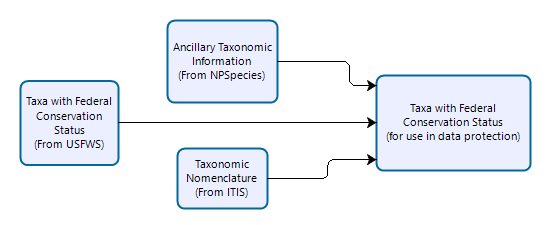
\includegraphics[width=7.64in]{vignettes/common/ProcessingWorkflow}

\begin{Shaded}
\begin{Highlighting}[]
\FunctionTok{sessionInfo}\NormalTok{()}
\end{Highlighting}
\end{Shaded}

\begin{verbatim}
## R version 4.3.2 (2023-10-31 ucrt)
## Platform: x86_64-w64-mingw32/x64 (64-bit)
## Running under: Windows 10 x64 (build 19045)
## 
## Matrix products: default
## 
## 
## locale:
## [1] LC_COLLATE=English_United States.utf8 
## [2] LC_CTYPE=English_United States.utf8   
## [3] LC_MONETARY=English_United States.utf8
## [4] LC_NUMERIC=C                          
## [5] LC_TIME=English_United States.utf8    
## 
## time zone: America/Denver
## tzcode source: internal
## 
## attached base packages:
## [1] stats     graphics  grDevices utils     datasets  methods   base     
## 
## other attached packages:
##  [1] QCkit_0.1.3           lubridate_1.9.3       forcats_1.0.0        
##  [4] stringr_1.5.1         dplyr_1.1.4           purrr_1.0.2          
##  [7] readr_2.1.4           tidyr_1.3.0           tibble_3.2.1         
## [10] ggplot2_3.4.4         tidyverse_2.0.0       devtools_2.4.5       
## [13] usethis_2.2.2         kableExtra_1.3.4.9000 yaml_2.3.8           
## [16] knitr_1.45            pander_0.6.5          rmarkdown_2.25       
## [19] markdown_1.11        
## 
## loaded via a namespace (and not attached):
##  [1] gtable_0.3.4      xfun_0.41         htmlwidgets_1.6.4 remotes_2.4.2.1  
##  [5] processx_3.8.2    tzdb_0.4.0        callr_3.7.3       vctrs_0.6.5      
##  [9] tools_4.3.2       ps_1.7.5          generics_0.1.3    parallel_4.3.2   
## [13] curl_5.2.0        fansi_1.0.6       pkgconfig_2.0.3   webshot_0.5.5    
## [17] lifecycle_1.0.4   compiler_4.3.2    munsell_0.5.0     httpuv_1.6.12    
## [21] htmltools_0.5.7   later_1.3.1       pillar_1.9.0      crayon_1.5.2     
## [25] urlchecker_1.0.1  ellipsis_0.3.2    cachem_1.0.8      sessioninfo_1.2.2
## [29] mime_0.12         tidyselect_1.2.0  rvest_1.0.3       digest_0.6.33    
## [33] stringi_1.8.3     fastmap_1.1.1     grid_4.3.2        archive_1.1.6    
## [37] colorspace_2.1-0  cli_3.6.2         magrittr_2.0.3    pkgbuild_1.4.2   
## [41] utf8_1.2.4        withr_2.5.2       prettyunits_1.2.0 scales_1.3.0     
## [45] promises_1.2.1    bit64_4.0.5       timechange_0.2.0  httr_1.4.7       
## [49] bit_4.0.5         png_0.1-8         hms_1.1.3         memoise_2.0.1    
## [53] shiny_1.8.0       evaluate_0.23     miniUI_0.1.1.1    viridisLite_0.4.2
## [57] profvis_0.3.8     rlang_1.1.2       Rcpp_1.0.11       xtable_1.8-4     
## [61] glue_1.6.2        xml2_1.3.6        pkgload_1.3.3     vroom_1.6.5      
## [65] svglite_2.1.2     rstudioapi_0.15.0 plyr_1.8.9        R6_2.5.1         
## [69] systemfonts_1.0.5 fs_1.6.3
\end{verbatim}

\begin{Shaded}
\begin{Highlighting}[]
\FunctionTok{Sys.time}\NormalTok{()}
\end{Highlighting}
\end{Shaded}

\begin{verbatim}
## [1] "2024-01-03 09:26:28 MST"
\end{verbatim}

\pagebreak

\hypertarget{appendix-b.-session-and-version-information}{%
\section{Appendix B. Session and Version
Information}\label{appendix-b.-session-and-version-information}}

In most cases you do not need to report session info (leave the
``session-info'' code chunk parameters in their default state:
eval=FALSE). Session and version information is only necessary if you
have set the ``Listing'' code chunk to eval=TRUE in appendix A. In that
case, change the ``session-info'' code chunk parameters to eval=TRUE.

\begin{verbatim}
## R version 4.3.2 (2023-10-31 ucrt)
## Platform: x86_64-w64-mingw32/x64 (64-bit)
## Running under: Windows 10 x64 (build 19045)
## 
## Matrix products: default
## 
## 
## locale:
## [1] LC_COLLATE=English_United States.utf8 
## [2] LC_CTYPE=English_United States.utf8   
## [3] LC_MONETARY=English_United States.utf8
## [4] LC_NUMERIC=C                          
## [5] LC_TIME=English_United States.utf8    
## 
## time zone: America/Denver
## tzcode source: internal
## 
## attached base packages:
## [1] stats     graphics  grDevices utils     datasets  methods   base     
## 
## other attached packages:
##  [1] QCkit_0.1.3           lubridate_1.9.3       forcats_1.0.0        
##  [4] stringr_1.5.1         dplyr_1.1.4           purrr_1.0.2          
##  [7] readr_2.1.4           tidyr_1.3.0           tibble_3.2.1         
## [10] ggplot2_3.4.4         tidyverse_2.0.0       devtools_2.4.5       
## [13] usethis_2.2.2         kableExtra_1.3.4.9000 yaml_2.3.8           
## [16] knitr_1.45            pander_0.6.5          rmarkdown_2.25       
## [19] markdown_1.11        
## 
## loaded via a namespace (and not attached):
##  [1] gtable_0.3.4      xfun_0.41         htmlwidgets_1.6.4 remotes_2.4.2.1  
##  [5] processx_3.8.2    tzdb_0.4.0        callr_3.7.3       vctrs_0.6.5      
##  [9] tools_4.3.2       ps_1.7.5          generics_0.1.3    parallel_4.3.2   
## [13] curl_5.2.0        fansi_1.0.6       pkgconfig_2.0.3   webshot_0.5.5    
## [17] lifecycle_1.0.4   compiler_4.3.2    munsell_0.5.0     httpuv_1.6.12    
## [21] htmltools_0.5.7   later_1.3.1       pillar_1.9.0      crayon_1.5.2     
## [25] urlchecker_1.0.1  ellipsis_0.3.2    cachem_1.0.8      sessioninfo_1.2.2
## [29] mime_0.12         tidyselect_1.2.0  rvest_1.0.3       digest_0.6.33    
## [33] stringi_1.8.3     fastmap_1.1.1     grid_4.3.2        archive_1.1.6    
## [37] colorspace_2.1-0  cli_3.6.2         magrittr_2.0.3    pkgbuild_1.4.2   
## [41] utf8_1.2.4        withr_2.5.2       prettyunits_1.2.0 scales_1.3.0     
## [45] promises_1.2.1    bit64_4.0.5       timechange_0.2.0  httr_1.4.7       
## [49] bit_4.0.5         png_0.1-8         hms_1.1.3         memoise_2.0.1    
## [53] shiny_1.8.0       evaluate_0.23     miniUI_0.1.1.1    viridisLite_0.4.2
## [57] profvis_0.3.8     rlang_1.1.2       Rcpp_1.0.11       xtable_1.8-4     
## [61] glue_1.6.2        xml2_1.3.6        pkgload_1.3.3     vroom_1.6.5      
## [65] svglite_2.1.2     rstudioapi_0.15.0 plyr_1.8.9        R6_2.5.1         
## [69] systemfonts_1.0.5 fs_1.6.3
\end{verbatim}

\begin{verbatim}
## [1] "2024-01-03 09:26:28 MST"
\end{verbatim}

\end{document}
